

\begin{figure}
    \centering
    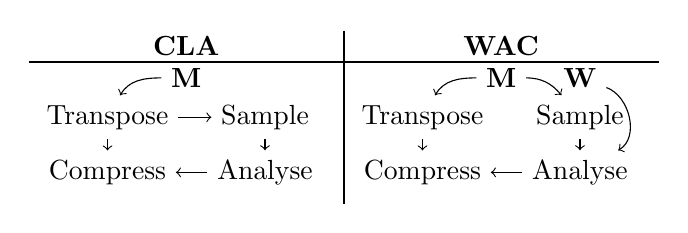
\begin{tikzpicture}

        \node(CLA) [xshift=-2.cm]{\textbf{CLA}};
        \node(WAC) [xshift=2.cm]{\textbf{WAC}};
        \draw[thick] (0,0.2) -- (0,-2);
        \draw[thick] (-4,-0.2) -- (4,-0.2);

        % CLA:
        \node(MCLA)[xshift=-2cm, yshift=-.4cm]{\textbf{M}};
        \node(TCLA)[xshift=-3.cm, yshift=-0.9cm]{Transpose};
        \draw[->] (MCLA) to [out=180, in=60] (TCLA); 
        \node(SCLA)[xshift=-1.cm, yshift=-0.9cm]{Sample};
        \draw[->] (TCLA) -- (SCLA);
        \node(ACLA)[xshift=-1.cm, yshift=-1.6cm]{Analyse};
        \draw[->] (SCLA) -- (ACLA);
        \node(CCLA)[xshift=-3.cm, yshift=-1.6cm]{Compress};
        \draw[->] (ACLA) -- (CCLA);
        \draw[->] (TCLA) -- (CCLA);

        % WAC:
        \node(MWAC)[xshift=2cm, yshift=-.4cm]{\textbf{M}};
        \node(WWAC)[xshift=3cm, yshift=-.4cm]{\textbf{W}};
        \node(TWAC)[xshift=1.cm, yshift=-0.9cm]{Transpose};
        \draw[->] (MWAC) to [out=180, in=60] (TWAC); 
        \node(SWAC)[xshift=3.cm, yshift=-0.9cm]{Sample};
        \draw[->] (MWAC) to [out=-0, in=130] (SWAC);
        \node(AWAC)[xshift=3.cm, yshift=-1.6cm]{Analyse};
        \draw[->] (SWAC) -- (AWAC);
        \draw[->] (WWAC) to [out=-20, in=30] (AWAC);
        \node(CWAC)[xshift=1.cm, yshift=-1.6cm]{Compress};
        \draw[->] (AWAC) -- (CWAC);
        \draw[->] (TWAC) -- (CWAC);

    \end{tikzpicture}
    \vspace{-0.4cm}
    \caption{Compression Phases Comparison}
    \Description[Compression Phases Comparison]{
        A Comparison of the compression phases showing that WAC skip trasposition before sampling
        allowing parallel workflows, and that WAC have two inputs A Matrix and a Workload.
    }
\end{figure}